\documentclass[tikz,border=8pt]{standalone}
% Shared look for every TikZ diagram. Load with % Shared look for every TikZ diagram. Load with % Shared look for every TikZ diagram. Load with \input{../../tools/tikz-style.tex}
\usepackage[T1]{fontenc}
\usepackage{lmodern}
\renewcommand{\sfdefault}{lmr}  % diagrams use the same serif as the text
\usetikzlibrary{arrows.meta, positioning, shapes.geometric, calc, fit, backgrounds}
\definecolor{cblue}{HTML}{4C78A8}
\definecolor{corange}{HTML}{F58518}
\definecolor{cgreen}{HTML}{54A24B}
\definecolor{cred}{HTML}{E45756}
\definecolor{cpurple}{HTML}{B279A2}
\definecolor{cgrey}{HTML}{6B6B6B}
\tikzset{
  every picture/.style={font=\sffamily, line width=1.2pt},
  box/.style={draw=#1, fill=#1!12, rounded corners=4pt, align=center, inner sep=7pt, minimum height=1.1cm},
  box/.default=cgrey,
  arrow/.style={-{Stealth[length=3mm]}, draw=cgrey, line width=1.4pt},
  title/.style={font=\sffamily\bfseries\Large},
  note/.style={font=\sffamily\small, text=cgrey, align=center},
}
\AtBeginDocument{\hyphenpenalty=10000 \exhyphenpenalty=10000}

\usepackage[T1]{fontenc}
\usepackage{lmodern}
\renewcommand{\sfdefault}{lmr}  % diagrams use the same serif as the text
\usetikzlibrary{arrows.meta, positioning, shapes.geometric, calc, fit, backgrounds}
\definecolor{cblue}{HTML}{4C78A8}
\definecolor{corange}{HTML}{F58518}
\definecolor{cgreen}{HTML}{54A24B}
\definecolor{cred}{HTML}{E45756}
\definecolor{cpurple}{HTML}{B279A2}
\definecolor{cgrey}{HTML}{6B6B6B}
\tikzset{
  every picture/.style={font=\sffamily, line width=1.2pt},
  box/.style={draw=#1, fill=#1!12, rounded corners=4pt, align=center, inner sep=7pt, minimum height=1.1cm},
  box/.default=cgrey,
  arrow/.style={-{Stealth[length=3mm]}, draw=cgrey, line width=1.4pt},
  title/.style={font=\sffamily\bfseries\Large},
  note/.style={font=\sffamily\small, text=cgrey, align=center},
}
\AtBeginDocument{\hyphenpenalty=10000 \exhyphenpenalty=10000}

\usepackage[T1]{fontenc}
\usepackage{lmodern}
\renewcommand{\sfdefault}{lmr}  % diagrams use the same serif as the text
\usetikzlibrary{arrows.meta, positioning, shapes.geometric, calc, fit, backgrounds}
\definecolor{cblue}{HTML}{4C78A8}
\definecolor{corange}{HTML}{F58518}
\definecolor{cgreen}{HTML}{54A24B}
\definecolor{cred}{HTML}{E45756}
\definecolor{cpurple}{HTML}{B279A2}
\definecolor{cgrey}{HTML}{6B6B6B}
\tikzset{
  every picture/.style={font=\sffamily, line width=1.2pt},
  box/.style={draw=#1, fill=#1!12, rounded corners=4pt, align=center, inner sep=7pt, minimum height=1.1cm},
  box/.default=cgrey,
  arrow/.style={-{Stealth[length=3mm]}, draw=cgrey, line width=1.4pt},
  title/.style={font=\sffamily\bfseries\Large},
  note/.style={font=\sffamily\small, text=cgrey, align=center},
}
\AtBeginDocument{\hyphenpenalty=10000 \exhyphenpenalty=10000}

\begin{document}
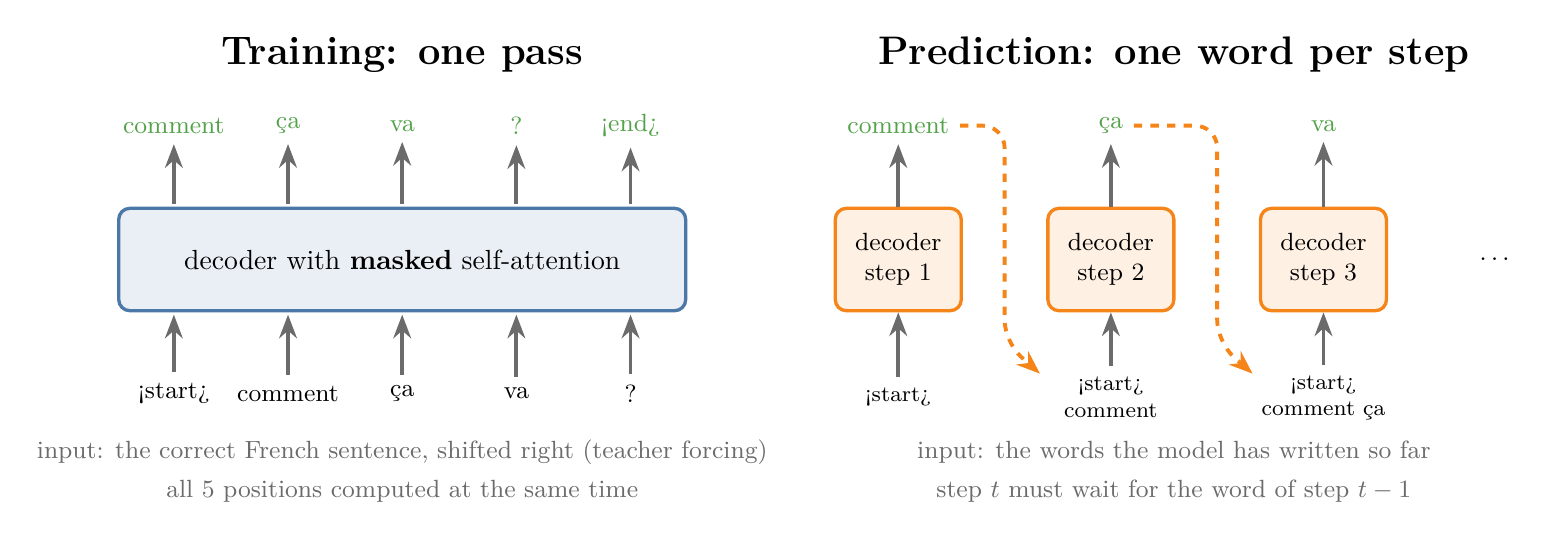
\begin{tikzpicture}[every node/.append style={font=\sffamily}]
  % ---------- training ----------
  \node[title] at (3.1, 4.6) {Training: one pass};
  \node[box=cblue, minimum width=7.2cm, minimum height=1.3cm] (dec) at (3.1, 2.0) {decoder with \textbf{masked} self-attention};
  \foreach \w [count=\i from 0] in {{<start>}, comment, ça, va, ?} {
    \node[font=\small] (in\i) at (0.2+1.45*\i, 0.3) {\w};
    \draw[arrow] (in\i) -- (0.2+1.45*\i, 1.3);
  }
  \foreach \w [count=\i from 0] in {comment, ça, va, ?, {<end>}} {
    \node[font=\small, text=cgreen] (out\i) at (0.2+1.45*\i, 3.7) {\w};
    \draw[arrow] (0.2+1.45*\i, 2.7) -- (out\i);
  }
  \node[note] at (3.1, -0.45) {input: the correct French sentence, shifted right (teacher forcing)};
  \node[note] at (3.1, -0.95) {all 5 positions computed at the same time};
  % ---------- inference ----------
  \node[title] at (12.9, 4.6) {Prediction: one word per step};
  \foreach \t/\inp/\out [count=\i from 0] in {1/{<start>}/comment, 2/{<start> comment}/ça, 3/{<start> comment ça}/va} {
    \node[box=corange, minimum width=1.6cm, minimum height=1.3cm, font=\small] (d\i) at (9.4+2.7*\i, 2.0) {decoder\\step \t};
    \node[font=\footnotesize, align=center, text width=1.9cm] (x\i) at (9.4+2.7*\i, 0.25) {\inp};
    \node[font=\small, text=cgreen] (y\i) at (9.4+2.7*\i, 3.7) {\out};
    \draw[arrow] (x\i) -- (d\i);
    \draw[arrow] (d\i) -- (y\i);
  }
  \draw[arrow, corange, dashed, rounded corners=8pt] (y0.east) -| (10.75, 0.95) -- (11.2, 0.55);
  \draw[arrow, corange, dashed, rounded corners=8pt] (y1.east) -| (13.45, 0.95) -- (13.9, 0.55);
  \node[font=\small] at (17.0, 2.0) {\dots};
  \node[note] at (12.9, -0.45) {input: the words the model has written so far};
  \node[note] at (12.9, -0.95) {step $t$ must wait for the word of step $t-1$};
\end{tikzpicture}
\end{document}
